\section{Branch prediction}

\begin{frame}[t]{Dynamic branch prediction}
\begin{itemize}
  \item Each conditional branch is \textmark{strongly biased}.
    \begin{itemize}
      \item Either is taken most of the time,
      \item or it is not taken most of the time.
    \end{itemize}

  \mode<presentation>{\vfill\pause}
  \item \textgood{Prediction based on execution profile}:
    \begin{itemize}
      \item Run once to collect statistics.
      \item Use the collected information to modify code and take advantage of information.
    \end{itemize}
\end{itemize}
\end{frame}

\begin{frame}[t]{Predictions with execution profile}
\begin{itemize}
  \item SPEC92: Branch frequency 3\% to 24\%
  \item \textgood{Floating point}:
    \begin{itemize}
      \item \textgood{Missprediction rate}. 
        \begin{itemize}
          \item \textmark{Average}: 9\%. 
          \item \textmark{Standard deviation}: 4\%.
        \end{itemize}
    \end{itemize}
  \item \textgood{Integer}:
    \begin{itemize}
      \item \textgood{Missprediction rate}. 
        \begin{itemize}
          \item \textmark{Average}: 15\%. 
          \item \textmark{Standard deviation}: 5\%.
        \end{itemize}
    \end{itemize}
\end{itemize}
\end{frame}

\begin{frame}[t]{Predictions with execution profile}
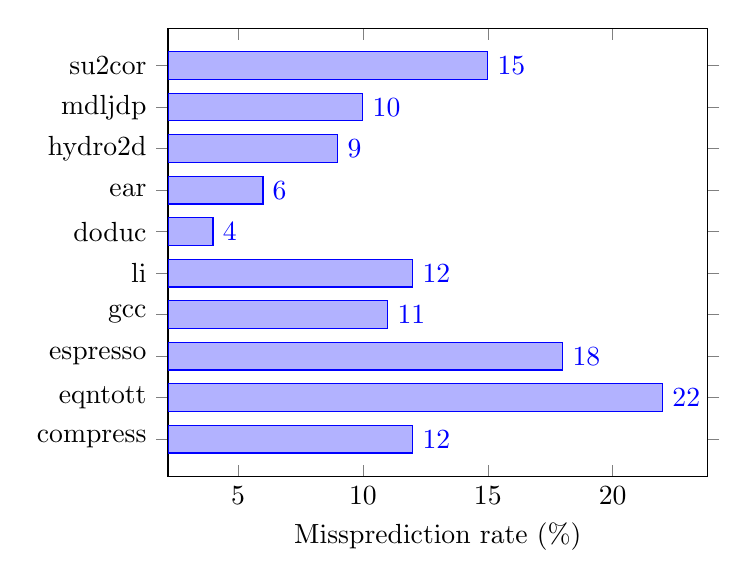
\begin{tikzpicture}
  \begin{axis}[
    xbar,
    xlabel={Missprediction rate (\%)},
    symbolic y coords={compress,eqntott,espresso,gcc,li,doduc,ear,hydro2d,mdljdp,su2cor},
    ytick=data,
    nodes near coords, nodes near coords align={horizontal},
    ]
    \addplot coordinates {
(12,compress) 
(22,eqntott)
(18,espresso)
(11,gcc)
(12,li)
(4,doduc)
(6,ear)
(9,hydro2d)
(10,mdljdp)
(15,su2cor)
};
  \end{axis}
\end{tikzpicture}
\end{frame}

\begin{frame}[t]{Dynamic prediction: BHT}
\begin{itemize}
  \item \textgood{Branch History Table}:
    \begin{itemize}
      \item \textmark{Index}: Lower bits of address (\textmark{PC}).
      \item \textmark{Value}: 1 bit (branch taken or not taken last time).
    \end{itemize}
  \mode<presentation>{\vfill}
  \item \textgood{Effects}:
    \begin{itemize}
      \item We don't know if the prediction is correct.
        \begin{itemize}
          \item Might come from another instrucciton located at different
                address with same lower bits.
        \end{itemize}
        \item Number of lower bits implies size of the buffer
          \begin{itemize}
            \item 10 lower bits $\Rightarrow$ 1024 entries.
          \end{itemize}
        \item If prediction fails bit is inverted
        \item \textbad{Drawback}: A loop branch fails twice.
          \begin{itemize}
            \item First and last iteration.
          \end{itemize}
    \end{itemize}
\end{itemize}
\end{frame}

\begin{frame}[t]{Dynamic prediction: BHT}
\begin{itemize}
  \item \textgood{Branch History Table}:
    \begin{itemize}
      \item \textmark{Index}: Lower bits of address (\textmark{PC}).
      \item \textmark{Value}: 2 bits. 
        \begin{itemize}
          \item \textgood{00} and \textgood{01}: Predict not taken.
          \item \textgood{10} and \textgood{11}: Predict taken.
        \end{itemize}
    \end{itemize}
\end{itemize}

\mode<presentation>{\pause}
\makebox[\textwidth][c]{
\input{en/m4-02-ilp/bht-statediag.tkz}
}
\begin{itemize}
  \item \textgood{Improvements}: Use more bits to improve precision.
\end{itemize}
\end{frame}

\begin{frame}[t,shrink=10]{BHT: Precision}
\begin{itemize}
  \item Missprediction rate:
    \begin{itemize}
      \item Wrong prediction in branch outcome.
      \item History of different branch in table entry.
    \end{itemize}
  \item BHT results of 2 bits and 4K entries:
\end{itemize}
\begin{tikzpicture}
  \begin{axis}[
    xbar,
    width=\textwidth, height=0.7\textheight,
    xlabel={Missprediction rate},
    symbolic y coords={li,eqntott,espresso,gcc,fpppp,spice,doduc,tomcatv,matrix300,nasa7},
    ytick=data,
    nodes near coords, nodes near coords align={horizontal},
    ]
    \addplot coordinates {
(10,li)
(18,eqntott)
(5,espresso)
(12,gcc)
(9,fpppp)
(9,spice)
(5,doduc)
(1,tomcatv)
(0,matrix300)
(1,nasa7)
};
  \end{axis}
\end{tikzpicture}
\end{frame}

\begin{frame}[t]{Dynamic branch prediction}
\begin{itemize}
  \item Why does branch prediction work?
    \begin{itemize}
      \item Algorithms exhibit regularities.
      \item Data structures exhibit regularities.
    \end{itemize}

  \mode<presentation>{\vfill}
  \item Is dynamic prediction better than static prediction?
    \begin{itemize}
      \item It looks like.
      \item There is a small number of important branches in programs with dynamic behavior.
    \end{itemize}
\end{itemize}
\end{frame}
